By Section \ref{Numerical methods for computing the Casimir energy}, to compute the Casimir energy, we need to evaluate 
$\log\frac{\det\mathsf{V}_{\mathrm{i}k}}{\det\tilde{\mathsf{V}}_{\mathrm{i}k}} = \log\det(\mathsf{V}_{\mathrm{i}k}\tilde{\mathsf{V}}_{\mathrm{i}k}^{-1})$ 
with different values of $k$. In this section, an efficient inverse-free and a LU decomposition based method will be introduced to compute this log determinant.

The log determinant of the matrix $\mathsf{V}_{\mathrm{i}k}\tilde{\mathsf{V}}_{\mathrm{i}k}^{-1}$ is equal to the sum of the logarithm of each eigenvalue of 
$\mathsf{V}_{\mathrm{i}k}\tilde{\mathsf{V}}_{\mathrm{i}k}^{-1}$. Since $\tilde{\mathsf{V}}_{\mathrm{i}k}$ is a compact perturbation of $\mathsf{V}_{\mathrm{i}k}$,
most of the eigenvalues are close enough to 1, which contributes nothing on the value of Casimir energy and this fact is shown in the Figure \ref{eigenvalues of VVtilde}.
Therefore, the computation process for the large-scale problem can become efficient if we only approximate the extreme eigenvalues 
which mainly contribute to the log determinant. In addition, we should also avoid directly computing the inverse of the matrix $\tilde{\mathsf{V}}_{\mathrm{i}k}$
since the computational complexity is cubic with respect to the matrix dimension.

In what follows, an inverse-free Krylov subspace method will be introduced to computed multiple smallest (or largest) eigenvalues of the generalized eigenvalue
problems simultaneously. Afterwards, we will discuss another efficient method based on $LU$ decomposition of the diagonal block matrix of $\tilde{\mathsf{V}}_{\mathrm{i}k}$. 
Finally, the comparison of these two methods will be shown.
\begin{figure}[H]
    \centering
    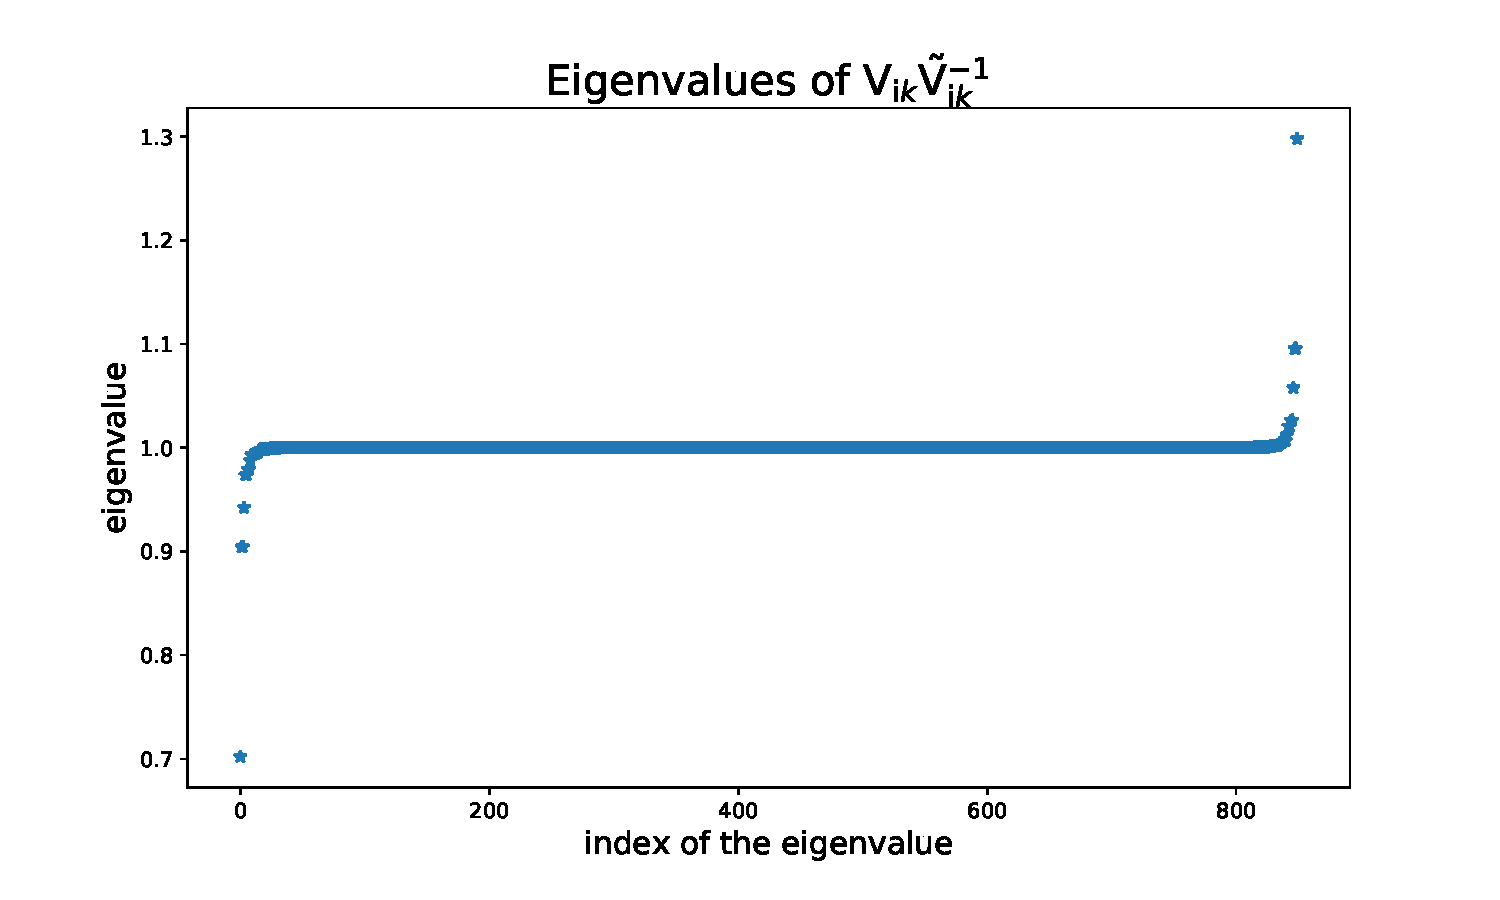
\includegraphics[scale = 0.5]{figures/eigenvalue_of_VVtilde.pdf}
    \caption{The eigenvalues of the matrix $\mathsf{V}_{\mathrm{i}k}\tilde{\mathsf{V}}_{\mathrm{i}k}^{-1}$ when $\mathrm{i}k = 0.8\mathrm{i}$.}
    \label{eigenvalues of VVtilde}
\end{figure}
\subsection{Method I: Krylov subspace for generalized eigenvalue problem}
Consider the eigenvalue problem: 
\begin{align} \label{EP}
    \mathsf{V}_{\mathrm{i}k}\tilde{\mathsf{V}}_{\mathrm{i}k}^{-1}\boldsymbol{x} = \lambda\boldsymbol{x},
\end{align}
where $\lambda$ is the eigenvalue and $\boldsymbol{x}$ is the corresponding eigenvalue. This eigenvalue problem is equivalent to the following generalized eigenvalue problem:
\begin{align}\label{GEP}
    \mathsf{V}_{\mathrm{i}k}\tilde{\boldsymbol{x}} = \lambda \tilde{\mathsf{V}}_{\mathrm{i}k}\tilde{\boldsymbol{x}}.
\end{align}
Thus, we can focus on solving the problem \eqref{GEP} instead of \eqref{EP} to avoid computing the matrix inversion. By \cite{quillen2010block}, the authors 
proposed an inverse-free Krylov subspace method for computing multiple eigenvalues of the symmetric definite generalized eigenvalue problem simultaneously 
and the following algorithm summarizes this method.
\begin{algorithm}[H]
    \SetAlgoLined
    Input: Symmetric matrix $A\in\mathbb{R}^{n\times n}$, s.p.d matrix $B\in\mathbb{R}^{n\times n}$ and a $B$-orthonormal matrix
    $X^{(1)} \in\mathbb{R}^{n\times p}$ with $X^{(1)*}BX = I_{p}$ and $m\geq 1$\\
    
    Output: The approximated $p$ smallest eigenvalues of $A\boldsymbol{x} = \lambda B\boldsymbol{x}$\\
    \begin{algorithmic}[1]
        \STATE Set $\Theta^{(1)} = \text{diag}(X^{(1)*}AX^{(1)})$
        \FOR {$k = 1, 2, \dots$} 
                \FOR {$i = 1, 2, \dots, p$}
                    \STATE Construct a basis $\hat{Z_{i}}$ of the $i$th Krylov subspace $K_{m}(A - \theta_{i}^{(k)}B, x_{i}^{(k)})$ with dimension $m$
                    \STATE Orthonormalize $\left[\hat{Z_{1}} \cdots \hat{Z_{p}}\right]$ to obtain $Z$
                    \STATE Project $A$ and $B$ on $Z$: $A_{m} = Z^{*}AZ$, $B_{m} = Z^{*}BZ$
                    \STATE Compute $p$ smallest eigenpairs $(\theta_{i}, u_{i})$, $1\leq i \leq p$ of the matrix pencil $(A_{m}, B_{m})$
                    \STATE $\Theta^{(k+1)} = \text{diag}(\theta_{1}, \dots, \theta_{p})$; $X^{(k+1)} = ZU$, $U = (u_{1} \cdots u_{p})$
                \ENDFOR
        \ENDFOR
        \end{algorithmic}
    \caption{Inverse-free Krylov subspace method for computing $p$ smallest eigenvalues of the generalized eigenvalue problem $A\boldsymbol{x} = \lambda B\boldsymbol{x}$}
    \label{Alg for computing the evals}
    \end{algorithm}
    
Algorithm \ref{Alg for computing the evals} can make us approximate $p$ smallest eigenvalues of the matrix pencil $(A,B)$ and the most trivial way to compute 
the $p$ largest eigenvalues is to use the same algorithm as above but only change the matrix $M$ to $-M$. Then we can find the $p$ smallest eigenvalues of 
$(-A, B)$ and by adding the negative sign in front of these eigenvalues, we can obtain $p$ largest eigenvalues of $(A, B)$.

We denote the $p$ smallest (or largest) eigenvalues obtained from this method as 
\begin{align}
    \Lambda_{\text{inv\_free}}^{\text{smallest}} = \left\{\lambda_{0}^{(s)}, \lambda_{1}^{(s)}, \dots, \lambda_{p-1}^{(s)}\right\},\label{smallest Eigevalues in Krylov}\\
    \Lambda_{\text{inv\_free}}^{\text{largest}} = \left\{\lambda_{0}^{(l)}, \lambda_{1}^{(l)}, \dots, \lambda_{p-1}^{(l)}\right\}. \label{largest Eigevalues in Krylov}
\end{align}
Then, the value of  $\log\det(\mathsf{V}_{\mathrm{i}k}\tilde{\mathsf{V}}_{\mathrm{i}k}^{-1})$ can be approximated by 
\begin{align*}
    \log\det(\mathsf{V}_{\mathrm{i}k}\tilde{\mathsf{V}}_{\mathrm{i}k}^{-1}) \approx \sum_{i = 0}^{p} \log\left(\lambda_{i}^{(s)}\right) + \sum_{i = 0}^{p} \log\left(\lambda_{i}^{(l)}\right)
\end{align*}

\subsection{Method II: $LU$ decomposition for inverting the matrix}
Another inverse-free way to compute $\log\det(\mathsf{V}_{\mathrm{i}k}\tilde{\mathsf{V}}_{\mathrm{i}k}^{-1})$ is to find the $LU$ decomposition for 
each diagonal block matrix and solve the linear system on each subdomain. To be specific, the inverse of the matrix $\tilde{\mathsf{V}}_{\mathrm{i}k}$ is
\begin{align*}
    \tilde{\mathsf{V}}_{\mathrm{i}k}^{-1} =  \tilde{\mathsf{V}}(\mathrm{i}k)^{-1} = \begin{bmatrix}
        \mathsf{V}_{11}(\mathrm{i}k) & 0      & \cdots & 0 \\
    0      & \mathsf{V}_{22}(\mathrm{i}k) & \cdots & 0\\
    \vdots & \vdots & \ddots & \vdots \\
    0      & 0      & \cdots & \mathsf{V}_{NN}(\mathrm{i}k) \\
\end{bmatrix}^{-1}
= \begin{bmatrix}
    \mathsf{V}_{11}^{-1}(\mathrm{i}k) & 0      & \cdots & 0 \\
0      & \mathsf{V}_{22}^{-1}(\mathrm{i}k) & \cdots & 0\\
\vdots & \vdots & \ddots & \vdots \\
0      & 0      & \cdots & \mathsf{V}_{NN}^{-1} (\mathrm{i}k)\\
\end{bmatrix}
\end{align*}

We can compute $LU$ decomposition of each diagonal block matrix $\mathsf{V}_{ii} = \mathsf{V}_{ii}(\mathrm{i}k)$ for $i = 1, 2, \dots, N$ and the decomposition is 
written as $\mathsf{V}_{ii} = \mathsf{L}_{ii}\mathsf{U}_{ii} $, where $\mathsf{L}_{ii}$ is a lower triangular matrix and $\mathsf{U}_{ii}$ is upper triangular.
Afterwards, we solve the linear system $\mathsf{L}_{ii}\mathsf{U}_{ii}\boldsymbol{x_{j}} = \boldsymbol{e}_{j}$, for $j = 1, 2, \dots, N_{\mathsf{V}_{ii}}$, where $\boldsymbol{e}_{j}$ 
denotes the vector with a 1 in the $j$th coordinate and 0's elsewhere and $N_{\mathsf{V}_{ii}}$ is the dimension of the block $\mathsf{V}_{ii}$. Finally, the inverse of $\mathsf{V}_{ii}$ is 
$\mathsf{V}_{ii}^{-1} = \begin{bmatrix}
    \boldsymbol{x}_{1} & \cdots & \boldsymbol{x}_{N_{\mathsf{V}_{ii}}}
\end{bmatrix}$ and we can notice that this whole process contains no step that needs us to compute the inverse of any matrix. 

We denote the inverse of the matrix $\tilde{\mathsf{V}}_{\mathrm{i}k}$ computed by the above inverse-free $LU$ decomposition method as 
$\tilde{\mathsf{V}}_{\mathrm{i}k}^{-1,\text{LU}}$ and to approximate multiple extreme eigenvalues of 
$\mathsf{V}_{\mathrm{i}k}\tilde{\mathsf{V}}_{\mathrm{i}k}^{-1,\text{LU}}$, we would like to firstly construct the Krylov subspace  
$K_{m}(\mathsf{V}_{\mathrm{i}k}\tilde{\mathsf{V}}_{\mathrm{i}k}^{-1,\text{LU}}, \boldsymbol{b})$, where $\boldsymbol{b}$ is some 
initial vector and $m$ is the dimension of this subspace. Afterwards, we implement the Arnoldi iteration to obtain the orthogonal basis of this $m$th Krylov 
subspace and project the matrix $\mathsf{V}_{\mathrm{i}k}\tilde{\mathsf{V}}_{\mathrm{i}k}^{-1,\text{LU}}$ onto this basis. 
This projection matrix is called the Hessenberg matrix and we denote it as $H_{m}$. By \cite{saad2011numerical}, the eigenvalues of $H_{m}$ (which are also 
called Ritz eigenvalues) can give good approximations to some eigenvalues of $\mathsf{V}_{\mathrm{i}k}\tilde{\mathsf{V}}_{\mathrm{i}k}^{-1,\text{LU}}$.
Therefore, we denote the the eigenvalues of $H_{m}$ as 
\begin{align}\label{Eigenvalues of Hessenberg}
    \Lambda_{\text{Arno}} = \left\{\lambda_{0}^{(\text{Arno})}, \lambda_{1}^{(\text{Arno})}, \dots, \lambda_{m-1}^{(\text{Arno})}\right\}
\end{align}
and the value of  $\log\det(\mathsf{V}_{\mathrm{i}k}\tilde{\mathsf{V}}_{\mathrm{i}k}^{-1})$ can be approximated by
\begin{align*}
    \log\det(\mathsf{V}_{\mathrm{i}k}\tilde{\mathsf{V}}_{\mathrm{i}k}^{-1}) \approx \sum_{i = 0}^{m-1}\log\left(\lambda_{i}^{(\text{Arno})}\right).
\end{align*}



%The rest of this section is to compare these two inverse-free methods.

\subsection{Comparison of two inverse-free methods}
Figure \ref{Method of GEP for m = 50} plots multiple smallest and largest approximated eigenvalues of the matrix $\mathsf{V}_{\mathrm{i}k}\tilde{\mathsf{V}}_{\mathrm{i}k}^{-1}$ when 
$p = 25$ (for $p$ in Method I) and the dimension of the Krylov subspace in both line four of Algorithm \ref{Alg for computing the evals} and Method II is $m = 50$.

\begin{figure}[H]
    \centering
    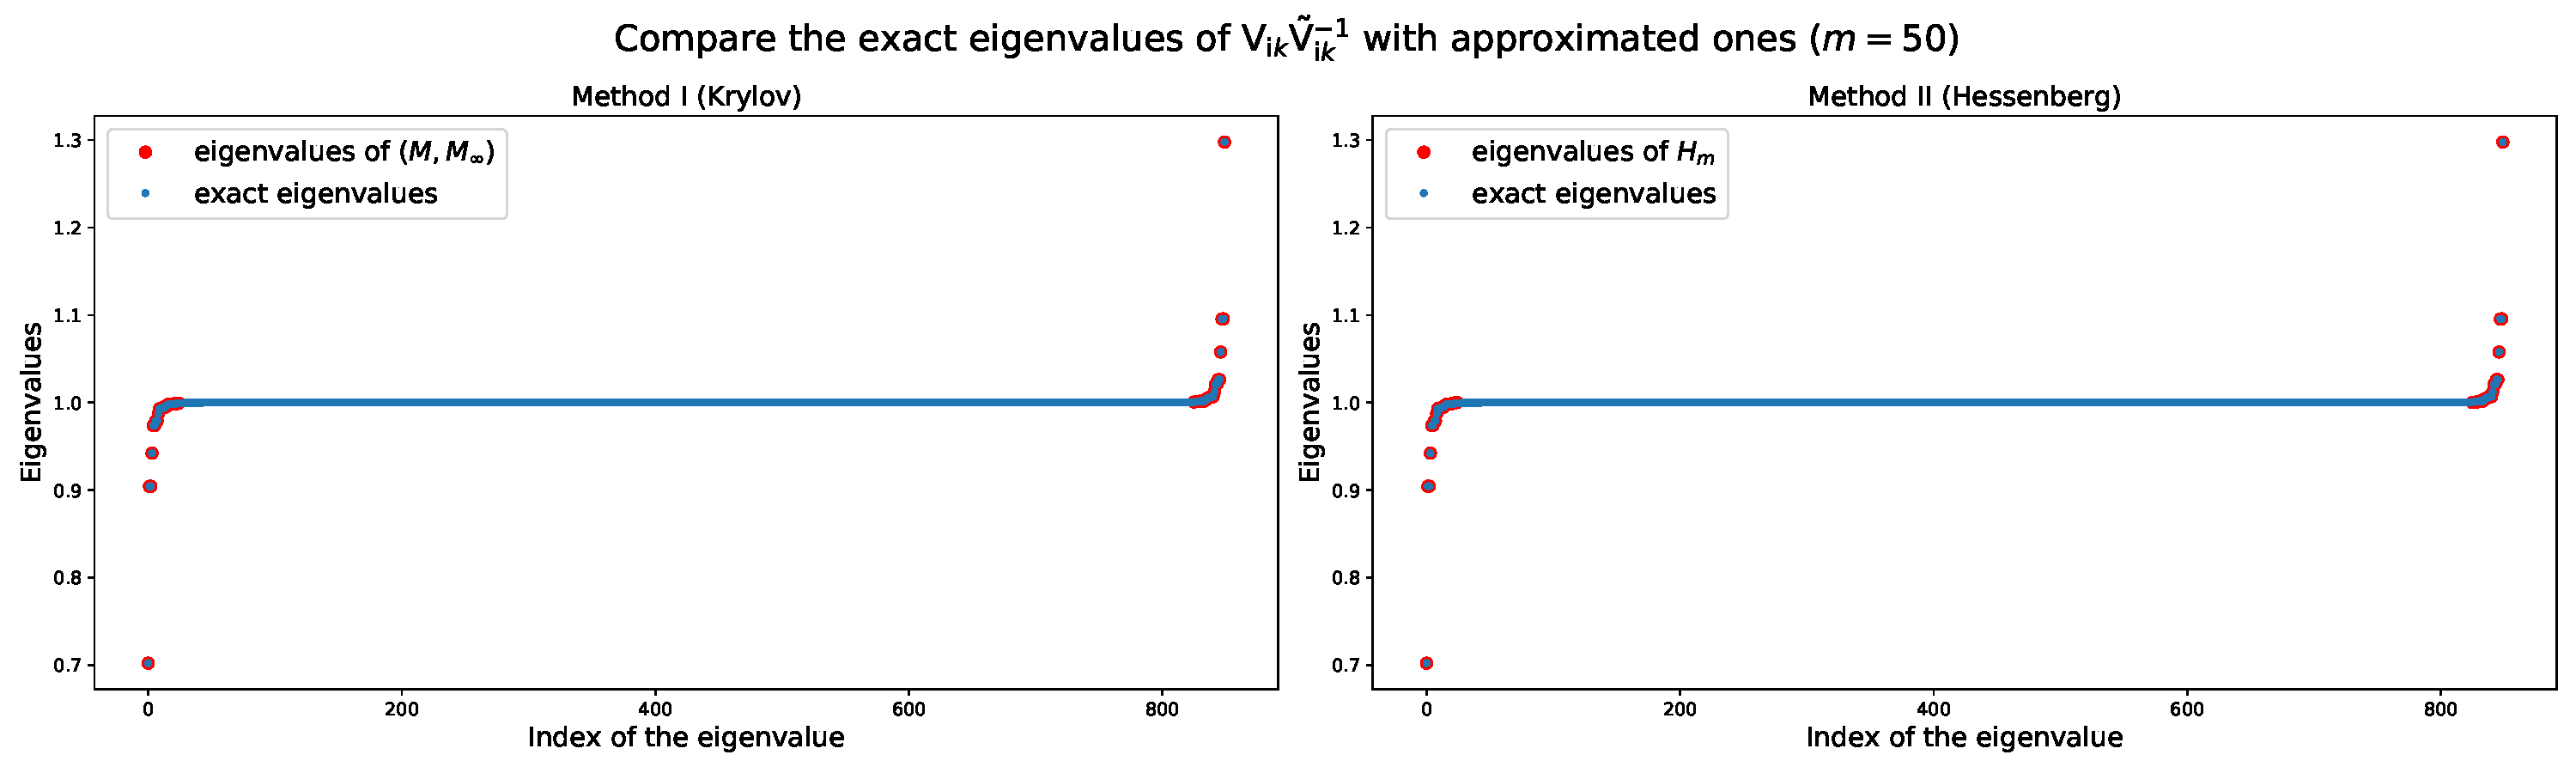
\includegraphics[scale = 0.36]{figures/Method_GEP_m_50.pdf}
    \caption{Comparison between $p$ approximated smallest eigenvalues and $p$ largest ones with the exact eigenvalues when $p = 25$ and the dimension of the 
    Krylov subspace in both line four of Algorithm \ref{Alg for computing the evals} and Method II is set as $m = 50$. }
    \label{Method of GEP for m = 50}
\end{figure}

By Figure \ref{Method of GEP for m = 50}, the approximated extreme eigenvalues are quite close to the exact ones and in order to see how close they are, we plot the
relative error between them in Figure \ref{relative error of GEP for m = 50}.
\begin{figure}[H]
    \centering
    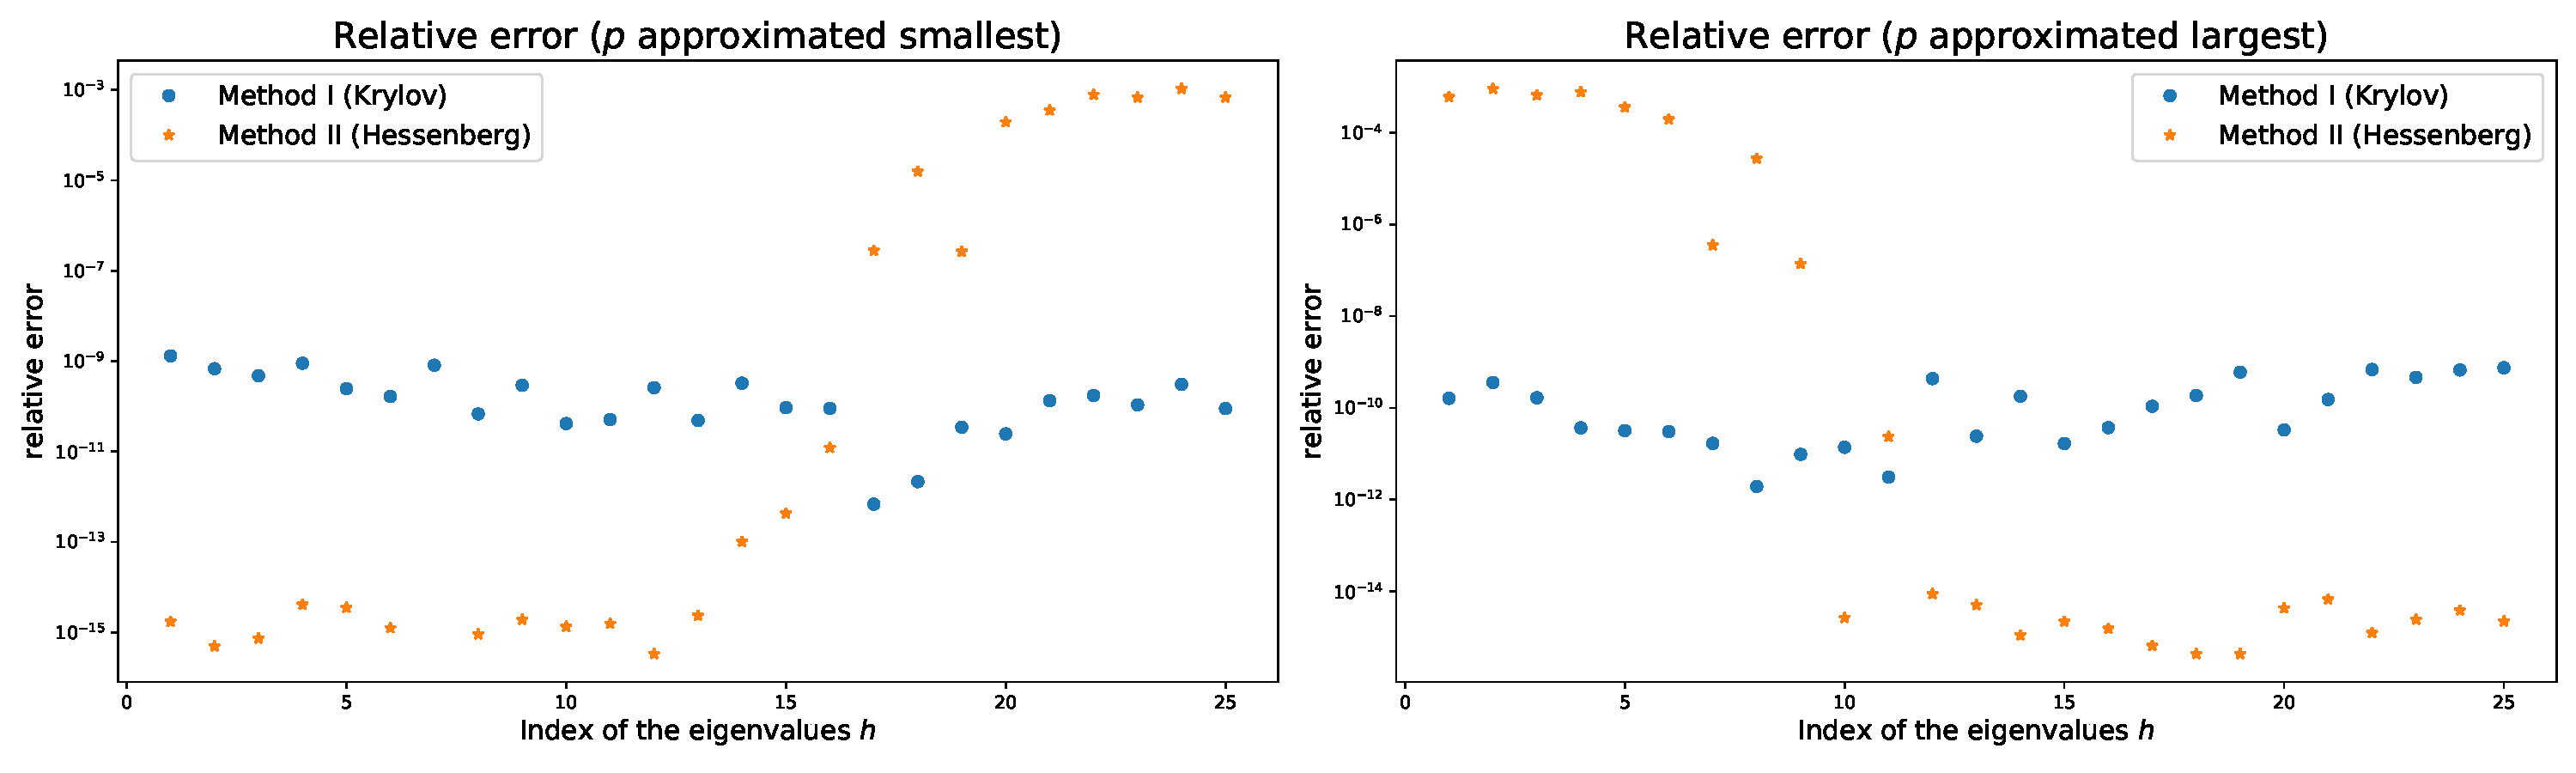
\includegraphics[scale = 0.36]{figures/rel_err_m_50.pdf}
    \caption{(Left) The relative error of the $p$ ($p = 25$) smallest eigenvalues between the exact and approximated ones. 
    (Right) The relative error of the $p$  ($p = 25$) largest eigenvalues between the exact and approximated ones.}
    \label{relative error of GEP for m = 50}
\end{figure}

To more intuitively see which inverse-free method is better, we would like to fix the dimension of the Krylov subspace as $m = 50$ and increase the number of 
the approximated eigenvalues from 2 to 50 and then plot the relative error in each case. The procedure is as follows.

For example, when the number of the approximated eigenvalue is 2, the relative error for the Method I (inverse-free) is computed by:
\begin{align*}
    \text{Err}^{(2)}_{\text{inv\_free}} = \frac{\left(\log(\lambda_{0}^{(s)}) + \log(\lambda_{p-1}^{(l)})\right) - \text{exact\_logdet}}{\text{exact\_logdet}},
\end{align*}
where \text{exact\_logdet} is the exact value of the log determinant of $\mathsf{V}_{\mathrm{i}k}\tilde{\mathsf{V}}_{\mathrm{i}k}^{-1}$ and  
$\lambda_{0}^{(s)}$, $\lambda_{p-1}^{(l)}$ are from the sorted sets $\Lambda_{\text{inv\_free}}^{\text{smallest}}$ in \eqref{smallest Eigevalues in Krylov} and 
$\Lambda_{\text{inv\_free}}^{\text{largest}}$ in \eqref{largest Eigevalues in Krylov}, respectively;
and the relative error for the Method II (standard Arnoldi) is computed by
\begin{align*}
    \text{Err}^{(2)}_{\text{Arno}} = \frac{\left(\log(\lambda_{0}^{\text{Arno}}) + \log(\lambda_{m-1}^{\text{Arno}})\right) - \text{exact\_logdet}}{\text{exact\_logdet}},
\end{align*}
where $\lambda_{0}^{\text{Arno}}$ and $\lambda_{m-1}^{\text{Hess}}$ are both from the sorted set $\Lambda_{\text{Arno}}$ in \eqref{Eigenvalues of Hessenberg}.

The following graph plots the relative error computed in both cases and we can see that their relative errors shares the same trend at the beginning and 
the Method II (Hessenberg) becomes worse when the number of the approximated eigenvalues becomes close to the dimension of the Krylov subspace.

\begin{figure}[H]
    \centering
    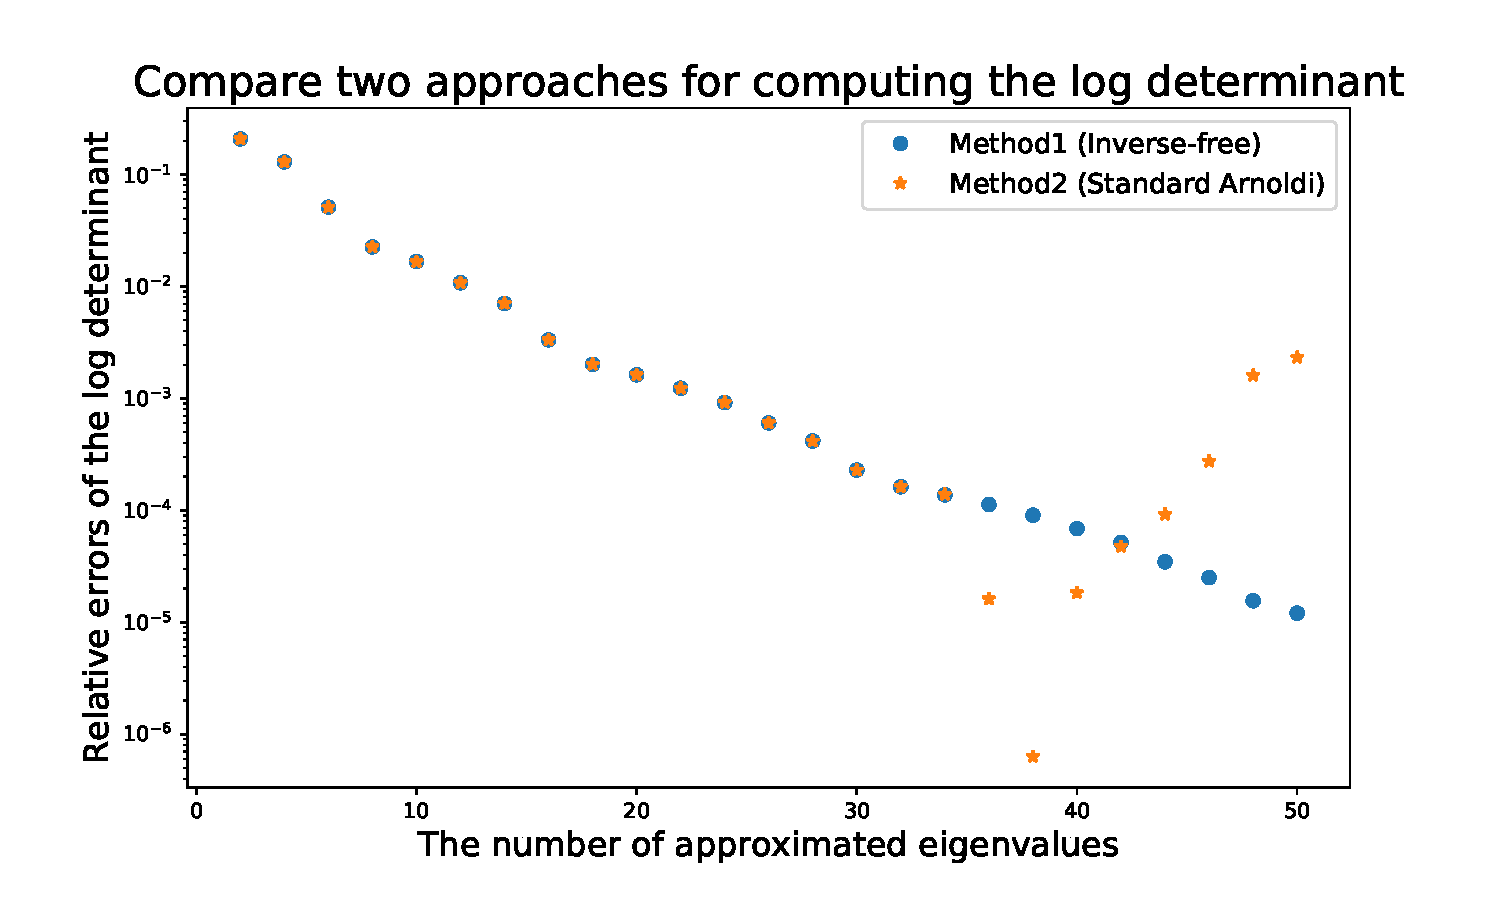
\includegraphics[scale = 0.5]{figures/compare_two_inv_free_approaches.pdf}
    \caption{The comparison between two inverse-free methods by fixing the dimension of the Krylov subspace as $m = 50$ and increasing the number of the 
    approximated eigenvalues from 2 to 50.}
\end{figure}
